% !TEX root=/home/tavant/these/manuscript/src/manuscript.tex

\section{Radial boundary conditions}
  \label{sec-DR-BC}
  
  In this section, we investigate the interaction between the azimuthal instability and the wall in the radial direction.
  
  \subsection{Impact of the wall on the oscillation}
  \label{subsec-kr}
  
  In the \ac{ECDI} dispersion relation described in \cref{sec-DR-kinetic}, the radial wavenumber is non-zero.
  Hence, in \cref{sec-DR-results}, we have chosen a wavelength that fits between the two walls.
  On the other hand, the oscillation seen in \cref{fig-phi_fluctuation_summary} seems not to present any oscillation in the radial direction.
  \Cref{fig-phi_osci_profile} shows the amplitude of the azimuthal instability on the plasma potential.
  It is defined as
  \begin{equation} \label{eq-stdphi}
    \delta \phi^2 = 2 \sigma_{\phi}^2 = \frac{{2}}{L_{\theta}} \int_0^{L_{\theta}} \lp  \phi - <\phi>_{\theta}  \rp ^2 d\theta,
  \end{equation}
  
  \begin{figure}[hbt]
    \centering
    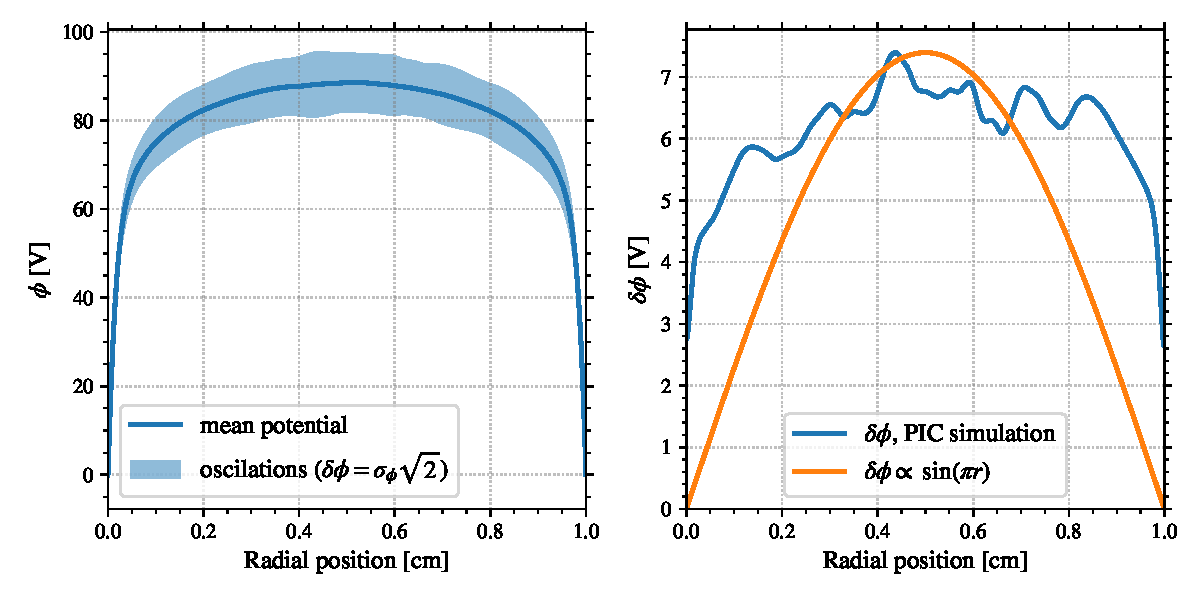
\includegraphics[width=\textwidth]{phi_oscillation}
    \caption{(Left) Radial profile of the mean plasma potential averaged in the azimuthal direction  and in time during the steady-state of the simulation ($t > 3.5 \,\micro\second$) and the average azimuthal instability amplitude. (Right) Radial profile of the  azimuthal instability amplitude, compared with a sinusoidal profile. }
    \label{fig-phi_osci_profile}
  \end{figure}
  
  
  We can see that the amplitude of the oscillation in the radial direction does not follow a sinusoidal profile.
  This observation contradicts the hypothesis made previously on the value of $k_r$.
  In order to better apprehend the radial profile of the instability amplitude, we show in \cref{fig-ratio} the ratio between $\delta \phi$ the fluctuation amplitude (showed on the right in \cref{fig-phi_osci_profile}) and $<\phi>_{\theta}$  the mean plasma potential (on the left in \cref{fig-phi_osci_profile}).
  
  \begin{figure}[hbt]
    \centering
    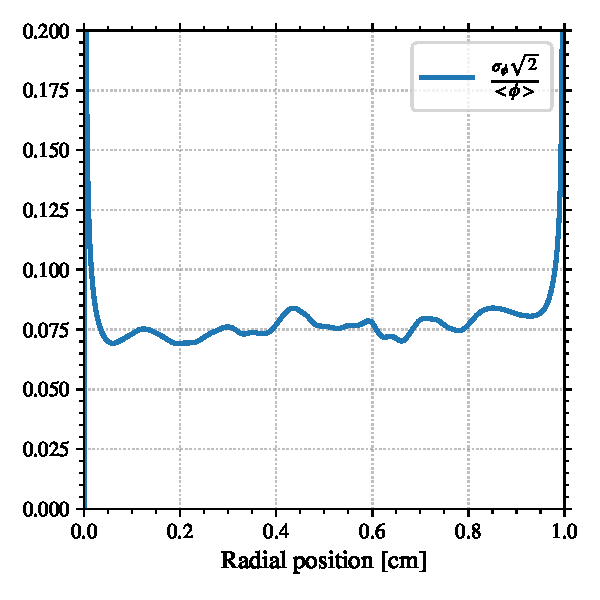
\includegraphics[width=\defaultwidth]{phi_oscillation_ratio}
    \caption{Radial profile of the ratio between $\delta \phi$ the fluctuation amplitude (showed on the right in \cref{fig-phi_osci_profile}) and $<\phi>_{\theta}$  the mean plasma potential (on the left in \cref{fig-phi_osci_profile}).}
    \label{fig-ratio}
  \end{figure}
  
  \Cref{fig-ratio} shows that the ration $\delta \phi / <\phi>$ is almost constant in the plasma, except close to the wall, where the plasma potential decreases much faster than the oscillations.
  The same behavior can bee observed in the profiles of the ion density, that can bee seen in \Cref{fig-ion_oscilation}.
  Actually, the behavior even more pronounced for the ion density, as they are not significantly affected by the wall.
  The ratio between the fluctuations and the mean value presents a radial profile almost constant.
  
  \begin{figure}[hbt]
    \centering
    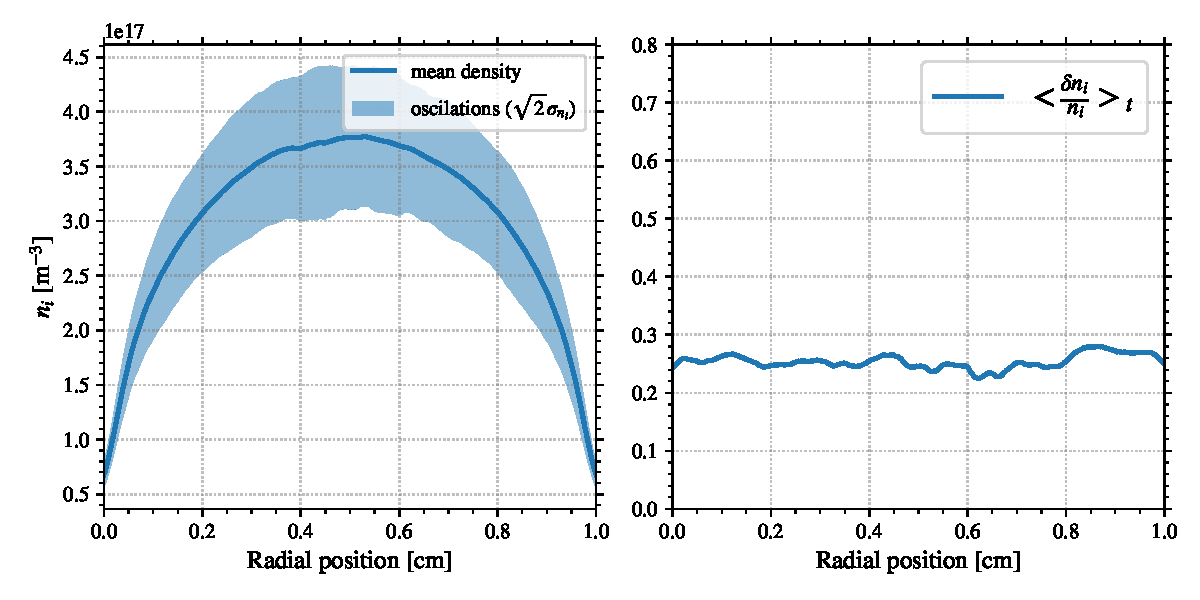
\includegraphics[width=\textwidth]{Ion_oscilations.pdf}
    \caption{Radial profile of (left) the mean ion density profile and $\delta n_i$ the fluctuation amplitude and (right) the ratio between $\delta n_i$ and $n_i$.}
    \label{fig-ion_oscilation}
  \end{figure}
  
  \vspace{1em}
  This may suggest that the sheaths screen significantly the wall from the oscillations, that are not affected by it.
  A screening of the wall have been observed in \citet{janhunen2018}, they observed radial structures that are not observed here.
  The difference between  \citet{janhunen2018} and the results presented here may be due to the difference in the radial length ($L_R =1 \,\centi\meter$ here against $L_R = 5.38\,\centi\meter$).
  
  As a conclusion, the interaction between the instability and the boundaries is not clearly understood.
  In addition, if there is no radial structure observed in our simulations, it means that the oscillation is purely azimuthally, or at least $\lde k_r <<1$.
  In this case, the cyclotron resonances should non-longer disappear \citep{ducrocq2006}, except due to non-linear demagnetisation, as discussed before \citep{boeuf2018,taccogna2019}.
  However, non-linear dispersion relations are out of the scope of the present work.
  
  
  \subsection{Impact of the electrostatic condition}
  \label{subsec-BC}
  \inlinenote{maybe this should be in Ch2: \\ Anne: yes }
  
  Let now observe the impact of the dielectric electrostatic boundary condition on the oscillation.
  We have see in \Cref{ch-2} that the dielectric boundary did not affect the simulation macroscopic results.
  \Cref{fig-closswallosci} shows the radial evolution in the first few cells of the amplitude of the oscillation of the azimuthal electric field on the left, and the ion density on the right, with grounded (metallic) wall and dielectric wall.
  
  \begin{figure}[hbt]
    \centering
    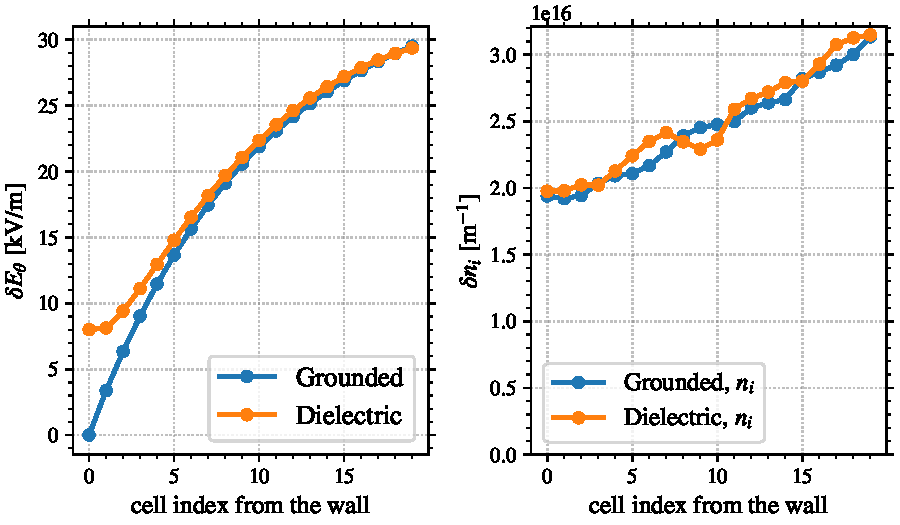
\includegraphics[width=\textwidth]{Ex_closewall.pdf}
    \caption{Radial evolution in the first cells of the amplitude of the oscillation of (left) the azimuthal electric field and (right) the ion density, with grounded (metallic) wall and dielectric wall.}
    \label{fig-closswallosci}
  \end{figure}
  
  We can see in \cref{fig-closswallosci} that the boundary condition do not affects the ion oscillations.
  This is consistent with the observation in \cref{subsec-kr} that the ion fluctuation was not affect by the wall.
  On the other hand, the azimuthal electric field has to go to zero when the wall is grounded.
  In contrast, the dielectric boundary condition, as modeled, allows a non-zero azimuthal electric field at the wall limit.
  However, the difference quickly disappears in the plasma.
  Hence, the electrostatic boundary condition induces only minor differences on the plasma discharge.
  
  